\documentclass{article}
\usepackage{color,graphicx,epstopdf}
\usepackage{amsmath,amssymb,amsthm}
\usepackage{xparse}
\usepackage
[
        a4paper,% other options: a3paper, a5paper, etc
        left=4cm,
        right=4cm,
        top=3cm,
        bottom=3cm,
]
{geometry}

% Document Settings
\pagenumbering{arabic}
\title{Linear Statistical Model Assignment 3 -- 2019}
\author{Maleakhi Agung Wijaya, 784091}
\date{Tutor: Qiuyi, Tuesday 3:15 PM}

%%%%%%%%%%%%%%%%%%%%%%%%%%%%%%%%%%%%%%%%%%%%%%%%%%%%%%%%%%%%%%%%%%
% Begin Document
\usepackage{Sweave}
\begin{document}
\maketitle
\Sconcordance{concordance:Assignment3.tex:Assignment3.Rnw:%
1 22 1 1 0 79 1 1 3 2 0 2 1 5 0 1 4 2 0 2 1 18 0 1 2 3 1 1 3 2 0 1 1 9 %
0 1 4 2 0 3 1 10 0 1 2 5 1 1 2 1 0 2 1 9 0 1 3 10 0 1 1 10 0 1 2 9 1 1 %
3 2 0 1 1 7 0 1 2 4 1 1 2 1 0 1 1 1 2 7 0 1 2 5 1 1 3 2 0 4 1 1 3 7 0 1 %
3 8 0 1 2 11 1 1 3 2 0 1 1 1 4 6 0 1 2 5 1 1 3 2 0 1 3 1 0 1 3 15 0 1 2 %
5 1 1 3 8 0 1 1 7 0 1 2 1 1 1 4 3 0 1 1 1 2 1 1 1 2 1 1 4 0 1 2 8 1 1 3 %
9 0 1 2 5 1 1 2 1 0 1 2 4 1 7 0 1 2 5 1 1 2 1 0 1 1 6 0 1 2 5 1 1 2 1 0 %
1 3 19 0 1 2 43 1 1 2 1 0 1 1 1 3 1 0 3 1 46 0 1 2 3 1}


% Question One
\section{Question One}
Let A be an $nxp$ matrix with $n \geq p$.

% Part a
\subsection{Part A}
\textit{\underline{Proof: }} $rank(A^cA) = rank(A)$ \\ \\
Using the property of rank, $rank(XY) \leq rank(X), rank(y)$ as well as definition of Conditional Inverse $AA^cA = A$, we can write the following inequalities:
\begin{eqnarray*}
  &\Rightarrow& rank(A) \geq rank(A^cA) \geq rank(AA^cA) \\
  &\Rightarrow& rank(AA^cA) = rank(A) \\
  &\therefore& rank(A) = rank(A^cA)
\end{eqnarray*}

\begin{flushright}
Q.E.D
\end{flushright}

% Part b
\subsection{Part B}
\textit{\underline{Proof: }} $I - A(A^TA)^cA^T$ is idempotent \\ \\
Start by multiplying the matrix with itself (assuming dimension conformed with each other), and if the result is the same with the original, then it is idempotent.
\begin{eqnarray*}
  &\Rightarrow& (I - A(A^TA)^cA^T)(I - A(A^TA)^cA^T) \\
  &\Rightarrow& = I - A(A^TA)^cA^T - A(A^TA)^cA^T + A(A^TA)^cA^TA(A^TA)^cA^T \\
  &\Rightarrow& = I - 2A(A^TA)^cA^T + A(A^TA)^cA^T \\
  &\therefore& = I - A(A^TA)^cA^T
\end{eqnarray*}

\begin{flushright}
Q.E.D
\end{flushright}

\noindent From line 2 to line 3, I use the property of Conditional Inverse such that $A(A^TA)^c(A^TA) = A$.

% Part c
\subsection{Part C}
\textit{\underline{Proof: }} $rank(I-A(A^TA)^cA^T) = n - rank(A)$ \\ \\
We will first prove that $I-A(A^TA)^cA^T$ is symmetric and idempotent matrix. From part (b), we know that this matrix is idempotent. Thus, we only need to prove for symmetric property. Here is proof that $I-A(A^TA)^cA^T$ is symmetric:
\begin{eqnarray*}
  &\Rightarrow& (I - A(A^TA)^cA^T)^T \\
  &\Rightarrow&  I^T - (A(A^TA)^cA^T)^T \\
  &\Rightarrow&  I - (A^T)^T((A^TA)^c)^TA^T \\
  &\Rightarrow&  I - A((A^TA)^T)^cA^T \\
  &\therefore&  I - A(A^TA)^cA^T
\end{eqnarray*}
\noindent Using the definition of symmetric matrix, we have shown that $(I - A(A^TA)^cA^T)^T = (I - A(A^TA)^cA^T)$ which implies that this matrix is symmetric. Since this matrix is symmetric and idempotent, we can use the Theorem 2.3 from Linear Algebra that rank = trace.
\begin{equation*}
  rank(I - A(A^TA)^cA^T) = trace(I - A(A^TA)^cA^T)
\end{equation*}

\noindent Next, notice that $A(A^TA)^cA^T$ is of dimension nxn. In addition, I will use some of the fundamental trace property from Linear Algebra below (i.e. trace(X+Y) = trace(X) + trace(Y)). Thus we can calculate as follows:
\begin{eqnarray*}
  &\Rightarrow& trace(I - A(A^TA)^cA^T) \\
  &\Rightarrow& trace(I) - trace(A(A^TA)^c(A^T)) \\
  &\Rightarrow& n - trace(A(A^TA)^c(A^T)) \\
  &\Rightarrow&  n - rank(A((A^TA)^T)^cA^T) \\
  &\therefore&  n - rank(A)
\end{eqnarray*}

\noindent From line 2 to line 3, as identity is of dimension nxn, therefore the trace is just the sums of the diagonal which equals to n. From line 3 to line 4, we notice that $A(A^TA)^c(A^T)$ is symmetric and idempotent as well (similar proof to proof above and part (b)), thus we can convert the trace back to rank by Theorem 2.3 again. Now from line 4 to line 5, we just need to show that $rank(A(A^TA)^cA^T) = rank(A)$. The lemma is shown below:

\begin{eqnarray*}
  rank(A(A^TA)^cA^T) \geq rank(A(A^TA)^cA^TA) = rank(A) \\
  rank(A) \geq rank(A(A^TA)^cA^T) \\
  \therefore rank(A(A^TA)^cA^T) = rank(A)
\end{eqnarray*}

\noindent $\therefore$ Using this small lemma, we have comlete/ justify the proof from earlier part and the rank of the respective matrix is $n-rank(A)$.
\begin{flushright}
Q.E.D
\end{flushright}

\section{Question 2}
We are interested in examining yield of tomato plants that have been grown with certain types of fertiliser. Here is the important variables in the model, such as X and y.

\begin{Schunk}
\begin{Sinput}
> # Response variable
> y <- c(43, 45, 47, 46, 48, 33, 37, 38, 35, 56, 54, 57)
> n <- length(y)
> print(y)
\end{Sinput}
\begin{Soutput}
 [1] 43 45 47 46 48 33 37 38 35 56 54 57
\end{Soutput}
\begin{Sinput}
> # Predictor Variable (Design matrix)
> X = matrix(c(rep(1, 12), rep(1,5), rep(0, 7), rep(0, 5), rep(1, 4), rep(0, 3), 
+              rep(0, 9), rep(1, 3)), 12, 4)
> r <- 3 
> print(X)
\end{Sinput}
\begin{Soutput}
      [,1] [,2] [,3] [,4]
 [1,]    1    1    0    0
 [2,]    1    1    0    0
 [3,]    1    1    0    0
 [4,]    1    1    0    0
 [5,]    1    1    0    0
 [6,]    1    0    1    0
 [7,]    1    0    1    0
 [8,]    1    0    1    0
 [9,]    1    0    1    0
[10,]    1    0    0    1
[11,]    1    0    0    1
[12,]    1    0    0    1
\end{Soutput}
\end{Schunk}

\subsection{Part A}
The conditional inverse is not unique (unless it is non-singular matrix). Theorem 6.2 from lecture can be used to find one of the conditional inverses. Here is the process of finding conditional inverse:

\begin{Schunk}
\begin{Sinput}
> # Calculate XTX
> XTX <- t(X) %*% X
> print(XTX)
\end{Sinput}
\begin{Soutput}
     [,1] [,2] [,3] [,4]
[1,]   12    5    4    3
[2,]    5    5    0    0
[3,]    4    0    4    0
[4,]    3    0    0    3
\end{Soutput}
\begin{Sinput}
> # Find XTXc using algorithm from lecture
> # Minor chosen is [5,0,0 ; 0,4,0; 0,0,3]
> XTXc <- matrix(0, 4, 4)
> XTXc[2:4, 2:4] = t(solve(XTX[2:4, 2:4]))
> XTXc <- t(XTXc)
> print(XTXc)
\end{Sinput}
\begin{Soutput}
     [,1] [,2] [,3]      [,4]
[1,]    0  0.0 0.00 0.0000000
[2,]    0  0.2 0.00 0.0000000
[3,]    0  0.0 0.25 0.0000000
[4,]    0  0.0 0.00 0.3333333
\end{Soutput}
\end{Schunk}

\noindent $\therefore$ Therefore, $(X^TX)^c$ is given by $\begin{bmatrix} 0 & 0 & 0 & 0 \\ 0 & 0.2 & 0 & 0 \\
0 & 0 & 0.25 & 0 \\ 0 & 0 & 0 & 0.33333 \end{bmatrix}$

\subsection{Part B}
Solution to the normal equation \textbf{b} can be calculated using $(X^TX)^cX^Ty$. Compute using R gives the following result:
\begin{Schunk}
\begin{Sinput}
> XTY <- t(X) %*% y
> b <- XTXc %*% XTY 
> print(b)
\end{Sinput}
\begin{Soutput}
         [,1]
[1,]  0.00000
[2,] 45.80000
[3,] 35.75000
[4,] 55.66667
\end{Soutput}
\begin{Sinput}
> # Find expression to another solutions
> print(b)
\end{Sinput}
\begin{Soutput}
         [,1]
[1,]  0.00000
[2,] 45.80000
[3,] 35.75000
[4,] 55.66667
\end{Soutput}
\begin{Sinput}
> print(diag(4) - XTXc %*% XTX)
\end{Sinput}
\begin{Soutput}
     [,1] [,2] [,3] [,4]
[1,]    1    0    0    0
[2,]   -1    0    0    0
[3,]   -1    0    0    0
[4,]   -1    0    0    0
\end{Soutput}
\end{Schunk}

\noindent Another solution to the normal equation that are computed using R code above is given below. Note that z here is arbitrary:
\begin{eqnarray*}
&\Rightarrow& b = (X^TX)^cX^Ty + [I-(X^TX)^cX^TX]z \\
&\Rightarrow& b = \begin{bmatrix} 0 \\ 45.8 \\ 35.75 \\ 55.67 \end{bmatrix} + \begin{bmatrix} 1 & 0 & 0 & 0 \\ -1 &0 &0 &0 \\ -1 &0 &0 &0 \\ -1 &0 &0 &0  \end{bmatrix}z \\
&\Rightarrow& b = \begin{bmatrix} z_1 \\ 45.8-z_1 \\ 35.75-z_1 \\ 55.67-z_1 \end{bmatrix}
\end{eqnarray*}

\subsection{Part C}
To check estimability, we use theorem from lecture and just check iff $t^T(X^TX)^cX^TX = t^T$. In this example, we will look at $4 \mu + 2 \tau_1 + \tau_2 + \tau_3$. R computation is shown as follows:
\begin{Schunk}
\begin{Sinput}
> # Check for estimability 4 mu + 2 tau1 + tau2 + tau 3
> t <- c(4, 2, 1, 1)
> print(t %*% XTXc %*% XTX)
\end{Sinput}
\begin{Soutput}
     [,1] [,2] [,3] [,4]
[1,]    4    2    1    1
\end{Soutput}
\end{Schunk}

\noindent $\therefore$ As we have that $t^T(X^TX)^cX^TX = t^T$, we know that $4 \mu + 2 \tau_1 + \tau_2 + \tau_3$ is estimable.

\subsection{Part D}
We want to calculate the prediction interval of the yield of a tomato plant on fertiliser 1. The prediction interval is formulated as $t^Tb \pm t_{\alpha/2} s \sqrt{1+t^t(X^TX)^ct}$.
\begin{Schunk}
\begin{Sinput}
> t <- c(1, 1, 0, 0)
> s2 <- sum((y-X%*%b)^2) / (n-r)
> print(t %*% b + c(-1, 1) * qt(0.975, n - r) * sqrt(s2) * 
+         sqrt(1 + t(t) %*% XTXc %*% t))
\end{Sinput}
\begin{Soutput}
[1] 40.96818 50.63182
\end{Soutput}
\end{Schunk}

\noindent $\therefore$ The prediction interval calculated using R gives [40.96818, 50.63182]

\subsection{Part E}
To test hypothesis that fertilisers 2 and 3 have no difference in yield, we can express the test as $H_0: C\beta = 0$, where C is given by $[0, 0, 1, -1]$. The test statistics for this test is given by $\frac{(Cb)^T[C(X^TX)^cC^T]^{-1}Cb / m}{SSRes / (n - r)}$. We know that m = 1 since the rank of C is 1 and $(n-r) = 9$. Performing the test using R gives the following result:

\begin{Schunk}
\begin{Sinput}
> # Perform hypothesis test (manual)
> C <- matrix(c(0,0,1,-1), 1, 4)
> m <- qr(C)$rank
> numerator <- (C%*%b)%*%solve(C%*%XTXc%*%t(C))%*%(C%*%b) / m
> denominator <- s2
> fstat<-numerator /denominator
> # Print f statistic
> print(fstat)
\end{Sinput}
\begin{Soutput}
         [,1]
[1,] 178.8633
\end{Soutput}
\begin{Sinput}
> # Print p-value
> pf(fstat, m, n-r, lower=F)
\end{Sinput}
\begin{Soutput}
             [,1]
[1,] 3.042802e-07
\end{Soutput}
\end{Schunk}

\noindent $\therefore$ From the result above, we know that p value is really small (less than 0.05), therefore we reject $H_0$ and conclude that fertilisers 2 and 3 have difference yield.

\newpage
\section{Question 3}

\newpage

\section{Question 4}
\subsection{Part A}
The data was plot using the following R command:

\begin{Schunk}
\begin{Sinput}
> # Read the data
> mile <- read.csv("data/mile.csv", header=TRUE)
> mile$Gender <- factor(mile$Gender) # Make the gender factor
> # Plot the data
> plot(Time ~ Year, data=mile, pch=as.character(Gender), 
+      col=ifelse(mile$Gender=="Male", 4, 2))
\end{Sinput}
\end{Schunk}
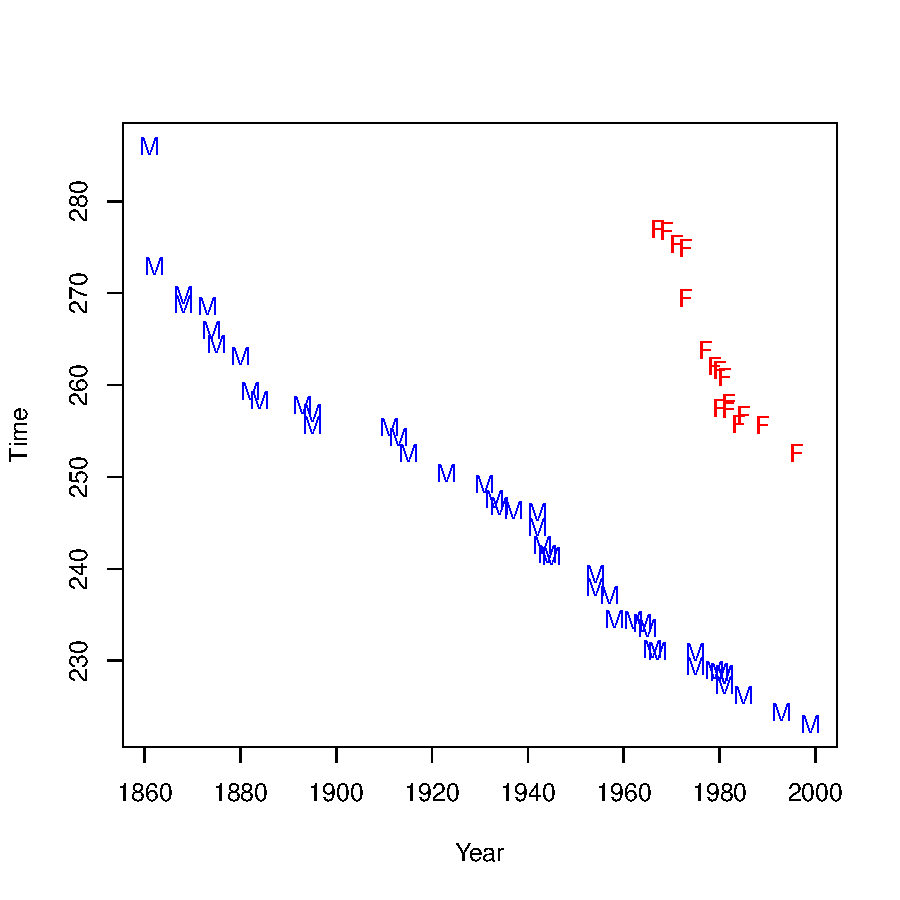
\includegraphics{Assignment3-007}

\noindent $\therefore$ Observing the male and female data, it can be seen that both data looks quite linear (downward trend). However, if we observe the record, it can only decrease. Therefore, the data are not independent and thus do not satisfy the linear model assumptions.

\subsection{Part B}
Looking at the model, we have 2 predictor variables which is gender and year. Hence, we will do an ANCOVA analysis since it is a mixture of categorical and continuous variable. We will compare the model with the interaction and the model without interaction (additive model) as shown in R code below:

\begin{Schunk}
\begin{Sinput}
> # Additive model
> amodel <- lm(Time ~ Year + Gender, data=mile)
> # Interactive model
> imodel <- lm(Time ~ Year * Gender, data=mile)
> # Perform ancova
> anova(amodel, imodel)
\end{Sinput}
\begin{Soutput}
Analysis of Variance Table

Model 1: Time ~ Year + Gender
Model 2: Time ~ Year * Gender
  Res.Df    RSS Df Sum of Sq      F    Pr(>F)    
1     59 895.62                                  
2     58 518.03  1    377.59 42.276 2.001e-08 ***
---
Signif. codes:  0 '***' 0.001 '**' 0.01 '*' 0.05 '.' 0.1 ' ' 1
\end{Soutput}
\end{Schunk}

\noindent $\therefore$ Based on our analysis using R above, we got a really low p-value. The anova tests that we do test if there is an interaction between factors. Based on the result, we can conclude that there is significant interaction and thus model with interaction is more appropriate.

\subsection{Part C}
Using R, we can inspect the coefficient of the interactive model to get the final fitted models for the male and female records. The code is given below:

\begin{Schunk}
\begin{Sinput}
> # Check coefficients of the interactive model
> print(imodel$coefficients)
\end{Sinput}
\begin{Soutput}
    (Intercept)            Year      GenderMale Year:GenderMale 
   2309.4247477      -1.0336960   -1355.6777866       0.6675093 
\end{Soutput}
\begin{Sinput}
> print(imodel$coefficients[c(1, 2)] + imodel$coefficients[c(3, 4)])
\end{Sinput}
\begin{Soutput}
(Intercept)        Year 
953.7469611  -0.3661867 
\end{Soutput}
\end{Schunk}
\noindent $\therefore$ Based on the result above, the regression for \textbf{female} is given by $Time = 2309 - 1.034 * Year$. For \textbf{male}, the regression line is given by $Time = 954 - 0.366 * Year$. Drawing this result in R gives the following new plot:

\begin{Schunk}
\begin{Sinput}
> # Plot regression line for both gender
> plot(Time~Year, data=mile,pch=as.character(Gender), 
+      col=ifelse(mile$Gender=="Male", 4, 2))
> year <- sort(mile$Year)
> time.female <- 2309 - 1.034 * year
> lines(year, time.female, col="red")
> time.male <-  954 - 0.366 * year
> lines(year, time.male, col="blue")
\end{Sinput}
\end{Schunk}
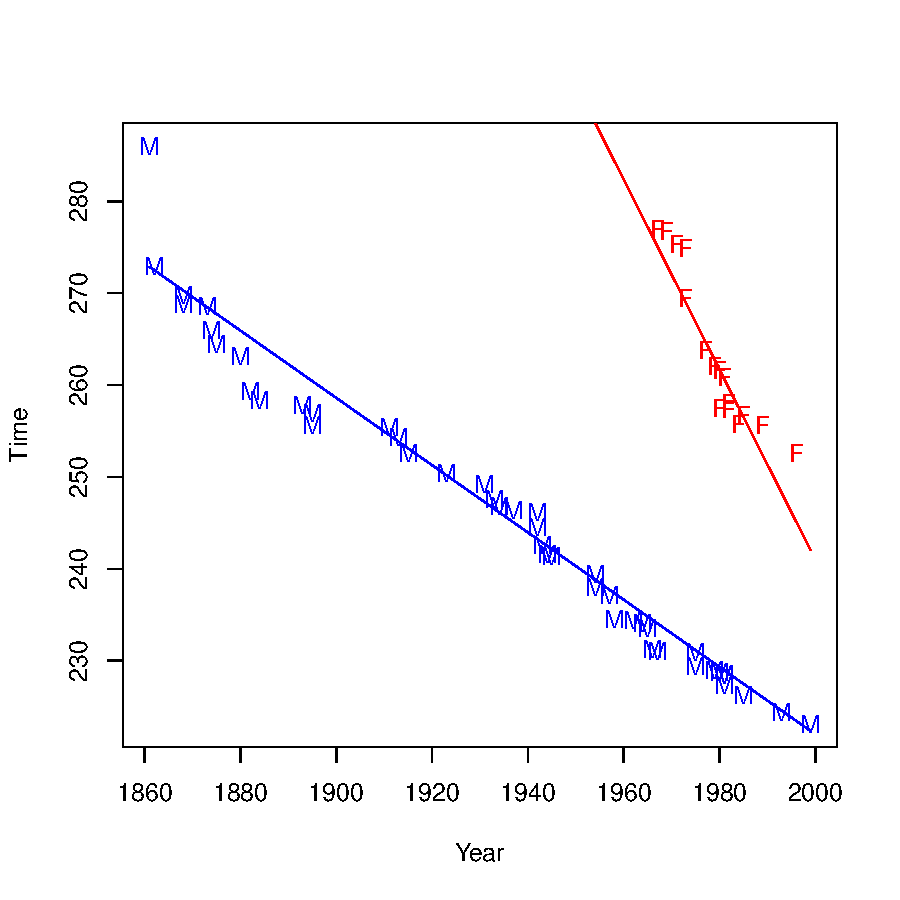
\includegraphics{Assignment3-010}

\subsection{Part D}
To calculate a point estimate for the year when the female world record will equal the male world record, we can equate male and female regression line as follow:

\begin{equation*}
  2309 - 1.034 * Year = 954 - 0.366 * Year
\end{equation*}

\noindent Calculation of this will be displayed in R as follows:
\begin{Schunk}
\begin{Sinput}
> # Solve the above equalities and round to the nearest integer for year
> print(round(-imodel$coefficients[3] / imodel$coefficients[4]))
\end{Sinput}
\begin{Soutput}
GenderMale 
      2031 
\end{Soutput}
\end{Schunk}

\noindent $\therefore$ Therefore, based on this result, we expect the year when female world record will be equal to male world record is in 2031. However, we cannot expect that this estimate to be accurate since we are extrapolating outside the range of the data.

\subsection{Part E}
Recall that the $\beta$ matrix is $\begin{bmatrix} \mu & \tau_1 & \tau_2 & \beta & \zeta_1 & \zeta_2 \end{bmatrix}^T$. Therefore to estimate when the male world record equals the female world record, we have that \textbf{t} is equals to $\begin{bmatrix} 0 & 1 & -1 & 0 & 0 & 0 \end{bmatrix}$. R code for testing is given below:

\begin{Schunk}
\begin{Sinput}
> library(MASS)
> year <- mile$Year
> X <- matrix(c(rep(1, 62), rep(1,46), rep(0, 16), rep(0, 46), rep(1, 16), year, year[1:46], rep(0, 16), rep(0, 46), year[47:62]), ncol=6)
> t <- c(0, 1, -1, 0, 0, 0)
> XTXc <- ginv(t(X) %*% X)
> print(round(t(t) %*% XTXc %*% t(X) %*% X))
\end{Sinput}
\begin{Soutput}
     [,1] [,2] [,3] [,4] [,5] [,6]
[1,]    0    0    0    0    0    0
\end{Soutput}
\end{Schunk}

\noindent From the result above $t^T(X^TX)^cX^TX \neq t^T$. Therefore by theorem from slide, we know that this quantity is not estimable and hence consistent with part (d).

\subsection{Part F}
The CI can be calculated as follow using R:

\begin{Schunk}
\begin{Sinput}
> s <- coef(summary(imodel))[, 2]
> print(imodel$coefficients[4] + c(-1, 1) * qt(0.975, df=58) * s[4])
\end{Sinput}
\begin{Soutput}
[1] 0.4620087 0.8730100
\end{Soutput}
\end{Schunk}

\noindent $\therefore$ Therefore the 95\% Confidence interval for the amount by which the hap between male and female world records narrow every year is (0.4620, 0.8730).

\subsection{Part G}
We can use linearHypothesis function to test if the slope of the male regression line is decreasing by 0.3 seconds each year. The following code is used to test this linearHypothesis.

\begin{Schunk}
\begin{Sinput}
> library(car)
> # Perform test
> linearHypothesis(imodel, c(0, 1, 0, 1), -0.3)
\end{Sinput}
\begin{Soutput}
Linear hypothesis test

Hypothesis:
Year  + Year:GenderMale = - 0.3

Model 1: restricted model
Model 2: Time ~ Year * Gender

  Res.Df    RSS Df Sum of Sq      F    Pr(>F)    
1     59 850.63                                  
2     58 518.03  1     332.6 37.238 9.236e-08 ***
---
Signif. codes:  0 '***' 0.001 '**' 0.01 '*' 0.05 '.' 0.1 ' ' 1
\end{Soutput}
\end{Schunk}

\noindent $\therefore$ Based on the result, we can reject the Null Hypothesis and conclude that the record decreases faster than 0.3.

\section{Question 5}
\subsection{Part A}
For this problem, we will use a completely randomised design for a single factor (treatment) with 3 levels. To test if the treatments are effective, we are going to compare with placebo ($\tau_3$). The study that we are going to conduct is $\tau_1 - \tau_3$ and $\tau_2 - \tau_3$. Apart from that, we also have a budget with the following constraint $5000n_1 + 2000n_2 + 1000n_3 = 100,000$. \\

\noindent To get the optimal allocation of the number of units to assign to each treatment we are going to minimise the function $f(n_1, n_2, n_3, \lambda)$ described below:
\begin{eqnarray*}
f(n_1, n_2, n_3, \lambda) = \sigma^2(\frac{1}{n_1} + \frac{1}{n_2} + \frac{2}{n_3}) + \lambda(\sum_{i=1}^3 n_i - n) 
\end{eqnarray*}

\noindent Then, we differentiate with respect to $n_i$ and equal it to 0 to get the optimal $n_i$. Similarly, later we will differentiate with respect to $n_3$. Differentiate with $n_i$ for $i = 1, 2$ gives the following expression:

\begin{eqnarray*}
    \frac{\partial f}{n_i} = \frac{-\sigma^2}{n_i^2} + \lambda = 0 \\
    \Rightarrow n_i^2 = \frac{\sigma^2}{\lambda}
\end{eqnarray*}

\noindent Now differentiate with respect to $n_3$, we get the following expression:
\begin{eqnarray*}
  \frac{\partial f}{n_3} = \frac{-2\sigma^2}{n_3^2} + \lambda = 0 \\
  \Rightarrow n_3^2 = \frac{2\sigma^2}{\lambda}
\end{eqnarray*}

\noindent Combining above result, we have that
\begin{eqnarray*}
  n_3^2 = 2n_1^2 = 2n_2^2 \\
  n_3 = \sqrt 2 n_1 =\sqrt2 n_2
\end{eqnarray*}

\noindent Hence, putting this value to our budget constraint, we have the following expression:
\begin{eqnarray*}
   7000n_i + 1000\sqrt 2 n_i = 100,000 \\
   \Rightarrow n_1 = n_2 = 12 \\
   \Rightarrow n_3 = 16
\end{eqnarray*}

\noindent $\therefore$ Therefore, the optimal allocation of the number of units to assign is 12 units for treatment 1, 12 units for treatment 2, and 16 units for treatment 3.


\subsection{Part B}
Randomization using R gives the following result:

\begin{Schunk}
\begin{Sinput}
> n <- c(12, 12, 16)
> nsum <- sum(n)
> # Randomize
> sample_number <- sample(1:nsum)
> treatment <- c(rep(1, 12), rep(2, 12), rep(3, 16))
> data <- data.frame(sample_number, treatment)
> print(data)
\end{Sinput}
\begin{Soutput}
   sample_number treatment
1             18         1
2             22         1
3              7         1
4             25         1
5             23         1
6              2         1
7             10         1
8             16         1
9             40         1
10            36         1
11            15         1
12            11         1
13            21         2
14            32         2
15            14         2
16            34         2
17            24         2
18            26         2
19             3         2
20             6         2
21            39         2
22             9         2
23            33         2
24            17         2
25            29         3
26            38         3
27            12         3
28            31         3
29            13         3
30            19         3
31            30         3
32            35         3
33             1         3
34            27         3
35             5         3
36            20         3
37            28         3
38            37         3
39             8         3
40             4         3
\end{Soutput}
\end{Schunk}

\noindent Here the dataframe produce indicating which sample number is given a particular treatment. The resulting data here is the result after randomization using sample function in R.

\end{document} 
